\documentclass[letterpaper,11pt]{article}
\pdfoutput=1
\usepackage{jinstpub}
\usepackage{lineno}
\usepackage[colorlinks=true]{hyperref}
\linenumbers

\title{Design and construction of MuTe: a hybrid Muon Telescope to study Colombian Volcanoes}

\author[a, 1]{J. Pe\~na-Rodr\'{\i}guez, \note{Corresponding author.}}
\author[a]{J. Pisco-Guabave}
\author[a,b]{D. Sierra-Porta}
\author[a]{M. Su\'arez-Dur\'an}
\author[c]{M. Arenas-Fl\'orez}
\author[c]{L. M. P\'erez-Archila}
\author[a]{J. D. Sanabria-G\'omez}
\author[d,e]{H. Asorey}
\author[a,f]{L. A. N\'u\~nez.}

\affiliation[a]{Escuela de F\'isica, Universidad Industrial de Santander,  Bucaramanga-Colombia.}
\affiliation[b]{Centro de Modelado Cient\'ifico, Facultad Experimental de Ciencias, Universidad del Zulia, Maracaibo-Venezuela.}
\affiliation[c]{Escuela de Ingenier\'ia Eléctrica, Universidad Industrial de Santander,  Bucaramanga-Colombia.}
\affiliation[d]{Laboratorio Detecci\'on de Part\'{\i}culas y Radiaci\'on, Instituto Balseiro y Centro At\'omico Bariloche, Comisi\'on Nacional de Energ\'{\i}a At\'omica, San Carlos de Bariloche-Argentina.}
\affiliation[e]{Sede Andina, Universidad Nacional de R\'io Negro, San Carlos de Bariloche-Argentina.}
\affiliation[f]{Departamento de F\'isica, Universidad de Los Andes, M\'erida-Venezuela.}


% e-mail addresses: only for the corresponding author
\emailAdd{jesus.pena@correo.uis.edu.co}


\abstract{We present a hybrid Muon Telescope designed and built for imaging active Colombian volcanoes. The MuTe has a resolution of tens of meters, low power consumption, robustness and transportability which make it suitable for using in difficult access zones where active volcanoes usually are. The main feature of MuTe is the implementation of a hybrid detection technique consisting in combining two scintillation panels for particle tracking and a Water Cherenkov Detector (WCD) for filtering background sources coming from the electromagnetic component of Extended Air Showers (EAS) and multiple particle events. We also show mechanical behavior of the MuTe during typical tremors and wind conditions at the observation place, as well as the frontend electronics design and power consumption.}

\keywords{Cosmic Rays, Muography, Volcanoes, Particle Identification, Noise Rejection}

\arxivnumber{xxxx.xxxxx} % only if you have one

% \collaboration{\includegraphics[height=17mm]{example-image}\\[6pt]
%   XXX collaboration}
% or

%\collaboration[c]{on behalf of XXX collaboration}


% if you write for a special issue this may be useful
%\proceeding{N$^{\text{th}}$ Workshop on X\\
%  when\\
%  where}



\begin{document}
\maketitle
\flushbottom
\section{Introduction}
\label{sec:intro}

Muography or Muon Radiography is a non-invasive technology whose primary purpose is to create digital images from density contrasts in the inner structure of objects from the atmospheric muon flux crossing through them \cite{Kaiser2019}. 

Muons are elementary particles two hundred times heavier than electrons, with a lifetime of approximately 2.2 $\mu$s., produced by the interaction of particles reaching the Earth's atmosphere from galactic and extragalactic sources.  These extraterrestrial impinging particles -- called cosmic rays-- generate showers of secondary other particles with a significant presence of muons, produced by charged pions and kaons decay processes. The energy spectrum of muons at sea level has a maximum of around 4 GeV with a flux of $\sim$ 1 cm$^{-2}$ min$^{-1}$ \cite{nakamura2010review}.


%According to the medium that one wants to study (a pyramid, a mountain, commercial container, etc.) more or less muons will cross according to density and thickness of the object. In order to have good resolution in the resulting density image we must to record many events making the measurements quite long before being processed. It should be noted that the muon flux is not uniform for all energies and also depends on the angle of detection.

The first muography was done by L. \'Alvarez et al. \cite{Alvarez1970} in 1969 to search for hidden chambers of the Pyramid of Chephren using spark chambers. The work was arduous since the detection time was of several days and the resolution and accuracy of the instrument were not as good as it had been desired, so despite researchers tenacity, the results were not of all satisfactory and the project was aborted. Nowadays, other applications concerned with the study of underground structures, such as natural caves \cite{caffau1997underground} or archaeological constructions \cite{basset2006mgr,menichelli2007scintillating} have been developed. However, muography of volcanoes has a particular interest \cite{tanaka2013subsurface,saracino2012looking,marteau2012muons,okubo2012imaging,lesparre2010geophysical,tanaka2007high, Bonomi2020, Bonechi2020}.

Despite a great deal of work in these areas, some particular problems have arisen and are still being addressed today:
\begin{itemize}

\item Muon flux penetrating volcano edifices is generally very weak, indeed, for a specific altitude above sea level at which the detector is located, the flux at angles close to the horizontal plane is roughly two orders of magnitude smaller than the flux for vertical muons and decreases about two orders of magnitude more considering muons that achieve to traverse the structure about 1 km-thick of standard rock \cite{groom2001muon, groom2000passage}. 


\item One of the major problems encountered so far in muography is related to background particles that are detected by the instrument but which do not come from the volcano, which means, they do not pass through the structure. Such background sources are composed of charged particles arriving from behind the detector \cite{jourde2013experimental}, EAS particles \cite{nishiyama2014experimental, Olah2017ICRC, KUSAGAYA2015, Bene2013, Olh2017}, and scattered low momentum muons ($<$ 1 GeV/c) \cite{nishiyama2016monte, Gomez2017, Olh2018, Olah2018Invest, ambrosino2015joint}. All of them generate signals that can be taken as true events implying an overestimation of penetrating particles flux with the consequence of a significant underestimation of the estimated density for the sight of the detector in the volcano. In fact, some anomalies in the expected particle flux have been found by several experiments e.g. an increase from 2 to 10 was measured by a scintillation detector at Mt. Etna \cite{carbone2013experiment}, whereas an excess from 4 to 8 was estimated using emulsion films at Mt. Showa-Shinzan \cite{nishiyama2016monte}.
\end{itemize}

%In fact, Carbone et. al. \cite{carbone2013experiment} found an increase in a factor from 2 to 10 in the measured particle flux by a scintillation detector, whereas Nishiyama et. al. \cite{nishiyama2016monte} found an excess from 4 to 8 in their measurements using emulsion films.


The muon telescope (MuTe) \cite{AsoreyEtal2017B, SierraPortaEtal2018} is a hybrid instrument suitable for the application of muography technique in different geophysical scenarios, with a particular interest in the study of internal structures of volcanoes. MuTe uses a hodoscope composed of plastic scintillator bars that determine the direction of particles passing through the detector and records the muon flux coming from the volcanic structure. Additionally, MuTe incorporates particle-identification techniques (PID) for reducing the background \cite{Bonechi2020, pena2019calibration}. A Water Cherenkov Detector (WCD) measures the energy loss of charged particles crossing the MuTe helping to filter the noise due to the soft-component of EAS (electrons and positrons), and particles arriving simultaneously. Discrimination of fake events due to scattered and backward muons is addressed using a picosecond Time-of-Flight system.

In this paper we describe a muon telescope designed for field experiments in volcanoes, addressing the two problems mentioned before. In section \ref{detector}, we present the MuTe detection characteristics. In section \ref{daq} we present the data acquisition system, trigger and power consumption of the MuTe. In section \ref{mechanical} we show simulations of the MuTe mechanical response for expected environmental conditions at volcanic areas. In section \ref{measurement} the first flux measurements carried out by the MuTe hodoscope and the estimation of background noise using the MuTe WCD are shown. Finally in section \ref{conclusions} we present the conclusions and remarks.

\section{The MuTe detector}
\label{detector}
In this section, we present the most significant characteristics of our muon telescope, MuTe: the event tracking and the signal-to-noise discrimination. Mainly our hybrid instrument consists of two detectors, i.e., a scintillator hodoscope and a WCD. This hybrid measurement technique had been previously implemented in the Pierre Auger Observatory to study the composition of primary cosmic rays \cite{martello2017pierre, aab2017muon, aab2016prototype}.

\subsection{Scintillator hodoscope: the tracking device}
Two detection panels, with 60 scintillator bars, implement the MuTe hodoscope. Each plastic scintillator strip is made of a polystyrene base of Styron 665-W doped with $1\%$ of $2,5$-diphenyloxazole (PPO) and $0.03\%$ of $1,4$-bis (5-phenyloxazol-2-yl) benzene (POPOP), co-extruded with a $0.25$ mm thick high reflectivity coating of $\text{TiO}_{\text{2}}$ \cite{PlaDalmau2003}. 

A wavelength shifting (WLS) fibre Saint-Gobain BCF-92 ($1.2$ mm diameter) is placed inside of a co-extruded tunnel of $1.8$ mm diameter. The fibre has a core refraction index of $1.42$, an absorption peak at $410$ nm, and an emission peak at $492$ nm. It captures the pulses produced by the crossing charged particles and drive them to a Silicon Photomultiplier (SiPM) Hamamatsu S13360-1350CS. The WLS fibre is centred in the SiPM sensitive area using a mechanical coupling (See Fig. \ref{fig:frame}). 

The scintillator panels build up an array of $30$ horizontal (X) and $30$ vertical (Y) bars reaching $900$ pixels of $16$ cm$^2$ active area each. The two X and Y scintillator layers are inside a $0.9$ mm thick stainless steel box, in conjunction with the SiPM electronics, the temperature/pressure sensors (HP03), and the coaxial cables for signal transmission. A second steel housing encapsulates the electronics readout, the ToF system, and the power supply, keeping all the components insulated and protected from environmental conditions. 

The hodoscope reconstructs the arrival direction of muons by taking into account the pairs of pixels activated in each panel. Changing the distance between the scintillator matrices varies the total aperture angle and the angular resolution of the telescope. The distance between the detector and the volcanic structure as well as the separation of the matrices define the spatial resolution of this telescope as
\begin{equation}
\Delta x=L\times\Delta\theta=L\times \arctan{\frac{2dD}{D^2+4d^2i(i+1)}},
\end{equation}
where $\Delta\theta$ is the angular resolution, $L$ is the distance to the target, $D$ is the separation between the panels, $d$ is pixel width, and $i$ is the $i$th illuminated pixel. For instance, for inter-matrix distances of $150$cm, $200$cm and $250$ cm, the total aperture angular is of $1.3$rad, $1.1$rad and $0.9$ rad for angular resolutions of $53$mrad, $40$mrad and $32$ mrad, respectively. Taking into account a distance to the volcano of $900$ m for the previous angular resolutions we will have spatial resolutions of $48$m, $36$m and $28$ m respectively.

\begin{figure}[htb]
\centering
\includegraphics[width=1\columnwidth]{Figures/panel.eps}
\caption{Mounting and coupling details for one detection panel. (Left) Mechanical assemble of the scintillator bar, the Saint-Gobain BCF-92 WLS fiber and the Hamamatsu S13360-1350CS SiPM. (Right) Scintillator panel with the SiPM electronics front-end and signal transmission cables (coaxial RG-174U).}
\label{fig:frame}
\end{figure}

\subsection{Telescope acceptance}
%\label{acceptan}
The acceptance of the instrument has an impact on the measured particle flux depending on telescope geometrical parameters: the number of pixels in the panels ($N_x \times N_y$), size of pixels ($d$), and separation of panels ($D$). Thus, the number of muons $N(\varrho)$ \cite{LesparreEtal2010}, can be defined as
\begin{equation}
N(\varrho)=\Delta T \times \mathcal{T}\times I(\varrho), \label{Nmuons}
\end{equation}
where $I(\varrho)$ is the integrated flux (measured in cm$^{-2}$ sr$^{-1}$ s$^{-1}$), $\mathcal{T}$ the acceptance function (measured in cm$^{2}$ sr), $\Delta T$ is the recording time, and $\varrho(L)$ represents the opacity parameter, related to the material muon absorption.

\begin{figure}[htb]
\centering
\includegraphics[width=0.48\columnwidth]{Figures/Solid_angle.png}
\includegraphics[width=0.48\columnwidth]{Figures/Aceptancia.png}
\caption{Angular resolution (left), and acceptance function (right) for the MuTe hodoscope with $N_x=N_y=30$, $d=4$ cm and $D=250$ cm in terms of each discrete direction. The maximum solid angle is $1.024\times 10^{-3}$ sr for perpendicular trajectories where the acceptance rises up to 3.69 cm$^{2}$ sr.}
\label{fig:acceptance}
\end{figure}

For a particular trajectory $r_{m,n}$ displayed by a pair of illuminated pixels on both panels, one can calculate the solid angle $\delta\Omega(r_{m,n})$ and the detection area $S(r_{m,n})$. All pairs of pixels with the same relative position, {$m=i-k$, $n=j-l$}, share the same direction, $r_{m,n}$ and the same $\delta\Omega(r_{m,n})$. This means directions normal to the hodoscope plane, have the larger detection area, while directions crossing corner-to-corner have the smaller solid angle and detection area. The acceptance is obtained \cite{LesparreEtal2010} multiplying the detection area by the angular resolution,
\begin{equation}
\mathcal{T}(r_{m,n})=S(r_{m,n})\times \delta\Omega(r_{m,n}).
\end{equation}

A telescope with two matrices of $N_x\times N_y$ pixels has $(2N_x-1)\times(2N_y-1)$ discrete directions $r_{m,n}$, spanning an solid angle $\Omega$. Our telescope equipped with 900 pixels is able to reconstruct 3481 discrete directions. In Fig. \ref{fig:acceptance}, we show the angular resolution and acceptance function for the Mute hodoscope with $N_x=N_y=30$ scintillator bars, size of pixel $d=4$ cm and $D=250$ cm. The total angular aperture of the telescope with that configuration is roughly 50$^{\circ}$(0.9 rad) with a maximum solid angle of $1.024\times 10^{-3}$ sr at $r_{0,0}$. On the other hand, the largest detection surface reaches $\approx 3.69$ cm$^{2}$ sr at $r_{0,0}$.

The MuTe acceptance can be compared with other telescopes for example described by \cite{UchidaTanakaTanaka2009space} with $N_x=N_y=12$, $d=7$ cm, and $D=100$ cm with a acceptance of $\mathcal{T}=30$ cm$^{2}$ sr and an angular resolution less than 0.018 sr, or with telescope presented in \cite{LesparreEtal2010} with $N_x=N_y=16$, $d=5$ cm, and $D=80$ cm with a acceptance of $\mathcal{T}=25$ cm$^{2}$ sr and an angular resolution less than 0.015 sr.

\subsection{Time-of-Flight: momentum measurement}

Time-of-Flight systems have been applied in muography to distinguish back-coming particles from those front-coming \cite{jourde2013experimental}. Particles entering from the rear side of the detector represent roughly 44$\%$ of background noise for zenith angles above 81$^{\circ}$ \cite{nishiyama2016monte}.

MuTe performs ToF measurements for identifying back-coming particles as well as low momentum ($<$ 1 GeV/c) muons which are scattered on the volcano contributing to the background noise. The MuTe ToF system was implemented on a Field Programming Gate Array (FPGA) employing a Time-to-Digital Converter (TDC). The TDC measures the time-lapse of crossing particles between the frontal and the rear panel with a time resolution of $\sim$ 40 ps.

\begin{figure}[htb]
\centering
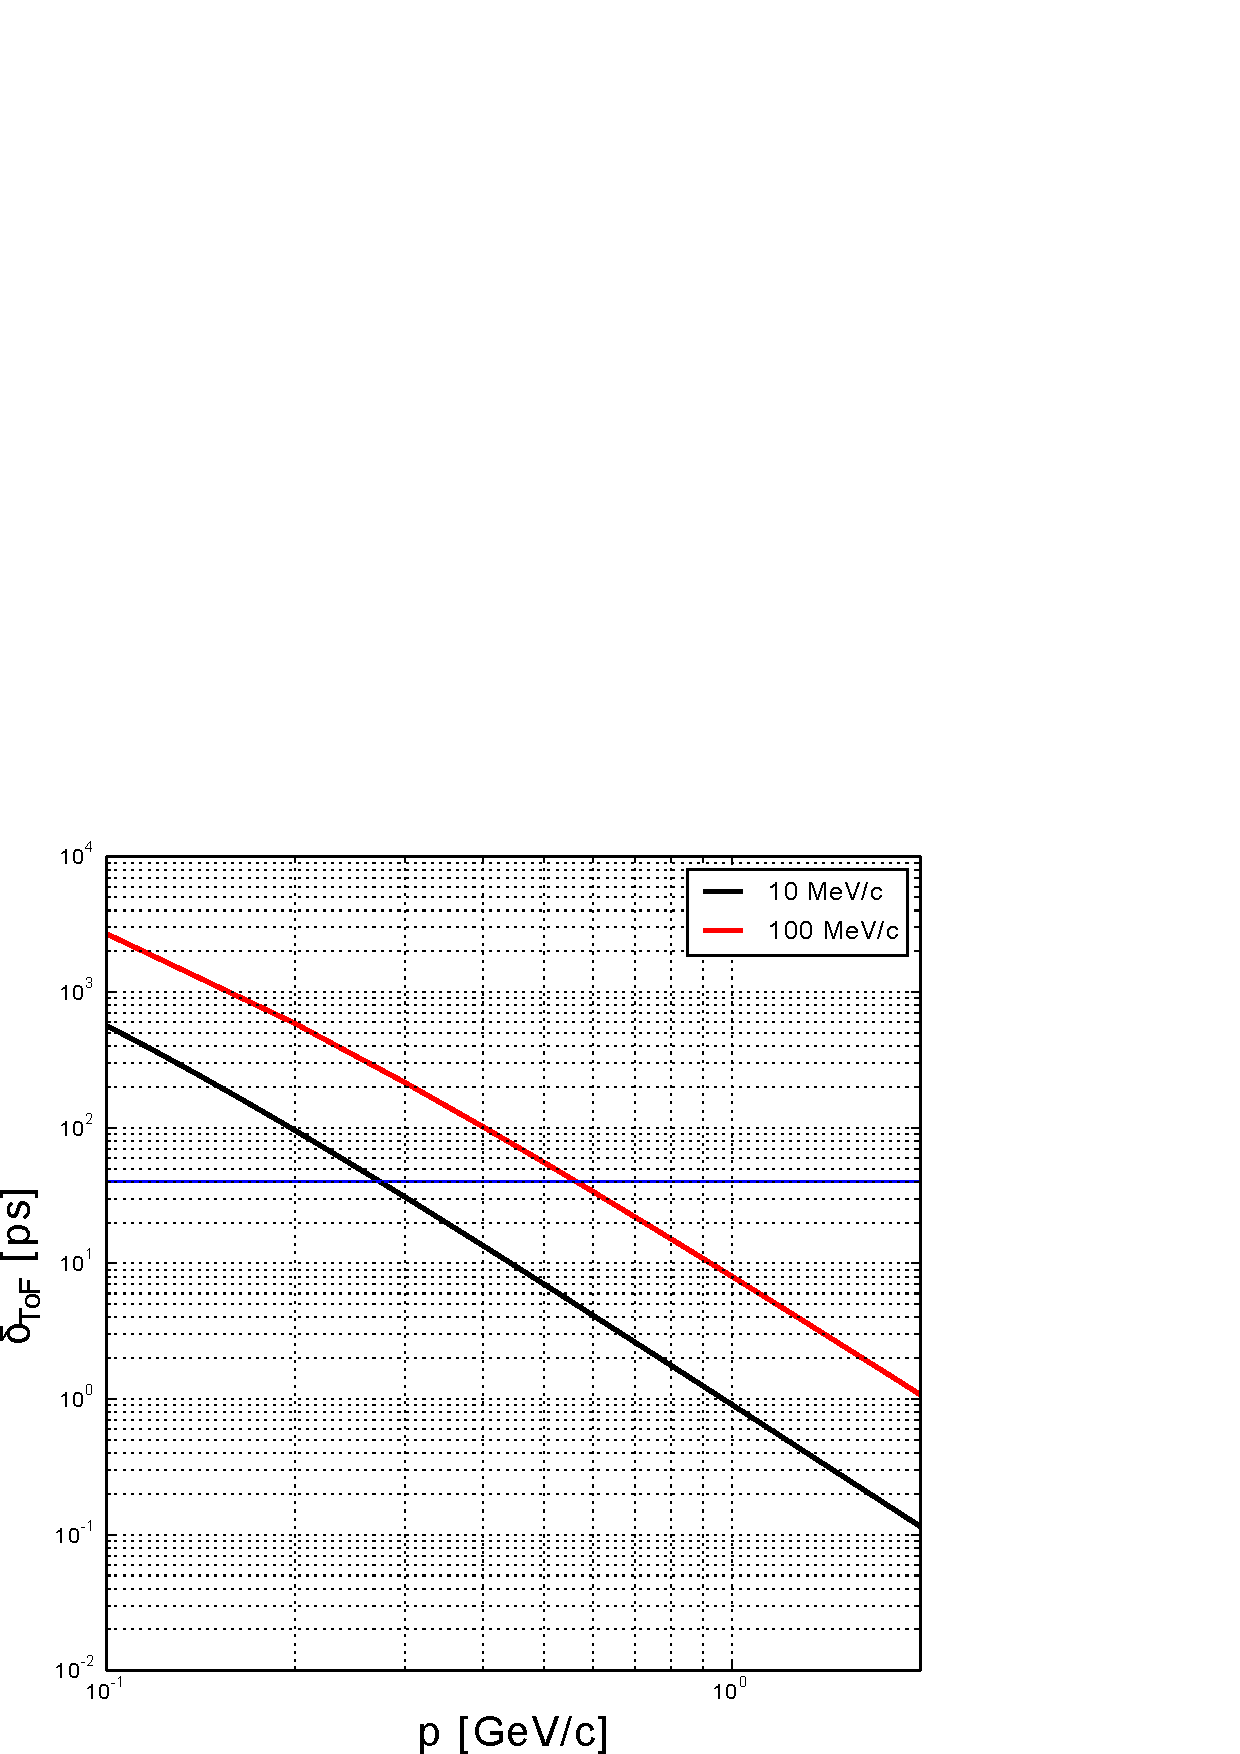
\includegraphics[width=0.5\columnwidth]{Figures/ToF_Resolution_250cm.png}
\caption{ToF resolution depending on the momentum estimation error, $\pm$10 MeV/c (black line) or $\pm$100 MeV/c (red line), for an inter-panel distance of 250 cm. The blue line represents the up-to-date MuTe ToF resolution (40 ps).}
\label{fig:ToF_Resolution}
\end{figure}

Taking into account the ToF $t$ of particles crossing the hodoscope in a given track $d$, and the particle identification provided by the WCD (distinguishing muons from electron/positrons) we can estimate particle momentum as follows
\begin{equation}
p = \frac{m_0 c d}{\sqrt{c^2t^2-d^2}}
\end{equation}
where $m_0$ is the mass of a charged particle at rest (105.65 Mev/c$^2$ for muons and 0.51 Mev/c$^2$ for electrons/positrons) and $c$ the speed of light. The momentum estimation uncertainty depends on the error of the ToF measurement and the error of the track length,
\begin{equation}
\sigma_p^2 = \left( \frac{\partial p}{\partial t} \right)^2 + \left( \frac{\partial p}{\partial d} \right)^2
\end{equation}

Measurement of momentum allows us to set a momentum threshold around $1$GeV/c above which the influence of noise due to soft muons is negligible \cite{nishiyama2016monte, nishiyama2014experimental, Olh2018, Olh2017, ambrosino2015joint}. In order to establish such a cutoff, we calculate the ToF resolution requirements, which depends on the momentum resolution we want to obtain. In Fig. \ref{fig:ToF_Resolution} we show the ToF resolution $\delta_t$ depending on the particle momentum for an estimation error of $\pm 10$ MeV/c and $\pm 100$ MeV/c considering an inter-panel distance of $2.5$ m. For perpendicular tracks to the hodoscope plane, we need a ToF resolution of $10$ ps to differentiate muons with momentum $> 1$ GeV/c with an error of $\pm 0.1$ GeV/c. With the actual $\sim 40$ ps resolution we can recognize muons under $0.6\pm 0.1$ GeV/c.

\subsection{Water Cherenkov Detector: deposited energy measurement}
Water Cherenkov Detectors, widely used in cosmic-ray observatories, has high acceptance, reasonable efficiency, and $\sim 100\%$ duty cycle. These devices made from few cubic meters of water with one or more photomultiplier tubes (PMTs), records the Cherenkov radiation produced by crossing charged particles with a velocity greater than the speed of light in this material. They are sensitive to the muonic and electromagnetic component of air showers \cite{Auger2015}. They also detect --indirectly-- high energy photons by pair production ($\gamma \rightarrow$ e$^{\pm}$) \cite{allard2007detecting, allard2008use, allekotte2008surface}. 

The MuTe's WCD is a $3.2$ mm thick stainless steel cube of $1.2$ m sides, coated inside with Tyvek diffuser sheets, which enhance interior reflectivity for the Cherenkov photons. An eight inches PMT --R5912 from Hamamatsu with a quantum efficiency of $22\%$ at $390$nm-- acts as the photosensitive device. The number of photons detected by the PMT can be associated with the deposited energy of the crossing particle allowing us to differentiate muons from the electromagnetic component of EAS (photons, electrons, and positrons) \cite{Billoir2014}. The EM component represents one of the most important noise sources in muography as is reported in several works \cite{KUSAGAYA2015, Nishiyama2014Noise, Marteau2012Noise}. At ground level, most probable muons ($\approx 4$ GeV) can traverse the whole WCD losing up to $240$ MeV (2 MeV/cm along 120 cm) for perpendicular trajectories, while the most probable electrons ($\approx$ 20 MeV) stops in only $10$cm of water losing 2 MeV/cm  \cite{groom2001muon,groom2000passage,lohmann1985energy,olive2014passage,Vasquez2018, Motta2018}.

The WCD detects charged particles coming from all directions due to its $2\pi$ acceptance with a deposited energy resolution of $\sim 0.72$ MeV and a measuring range from $50$ MeV to up $1.5$ GeV. This property allows the MuTe to monitor the local variations of the secondary particle flux over time \cite{Leon2018} and, to distinguish particles coming from the volcano direction by coincidence with the hodoscope trigger. 




\section{Electronics readout}
\label{daq}
The MuTe electronics has two main --independent but synchronized-- readout systems: one for the hodoscope and one for the WCD. 

\begin{figure}[htb]
\centering
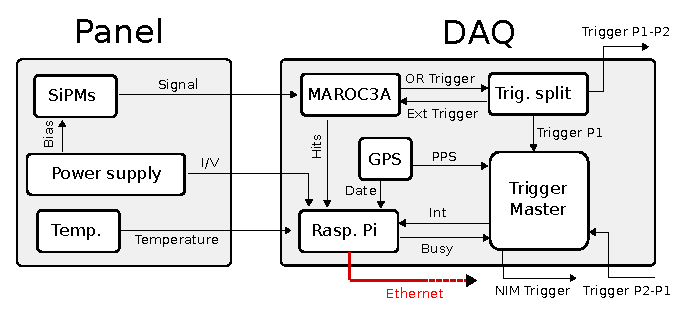
\includegraphics[width=0.8\columnwidth]{Figures/DAQ.eps}
\caption{Diagram of a single scintillator panel. Signals from the SiPMs are read out by the MAROC3 board whose slow control parameters are handled by a Raspberry Pi 2. All the detected events are time-stamped and sent via ethernet to the central monitoring server. The master trigger measures the ToF of the crossing particle and notifies the event truthfulness.}
  \label{fig:scintillatordetector1}
\end{figure}

In the hodoscope, $60$ SiPMs --S13360-1350CS, with a gain of $\sim 10^6$ and a photo-detection efficiency of $40\%$ at $450$nm-- detect the light signals coming from the scintillator bars. Each SiPM has a pre-conditioning electronics for amplifying ($\times 92$) and enhancing the signal-to-noise ratio before the transmission. 

A multi-channel ASIC MAROC3 from Omega discriminates the $60$ 
signals after making a gain adjustment to reduce the bar response variability. An FPGA Cyclone III sets the MAROC3 slow control parameters (channel gains and discrimination thresholds) from Altera. The discrimination threshold was set in $8$ photo-electrons taking into account previous analysis of the dark count, cross-talk and after-pulse of the SiPM S13360-1350CS \cite{Villafrades2020}.

The SCB Raspberry Pi 2 records the data from the scintillation panels when a coincidence condition is fulfilled (See \ref{trigger}). Environmental data (temperature, barometric pressure, and power consumption) is also recorded for post-processing, status monitoring, and calibration procedures. On the other hand, the SBC controls the SiPMs bias voltage depending on the temperature via the programmable power supply C11204. The recorded events are individually time-stamped with a resolution of 10 ns and synchronized using the PPS (Pulse Per Second) signal from a Venus GPS. A general diagram of the electronics readout for a single scintillator panel is shown in Fig. \ref{fig:scintillatordetector1}.

\begin{figure}[htb]
\centering
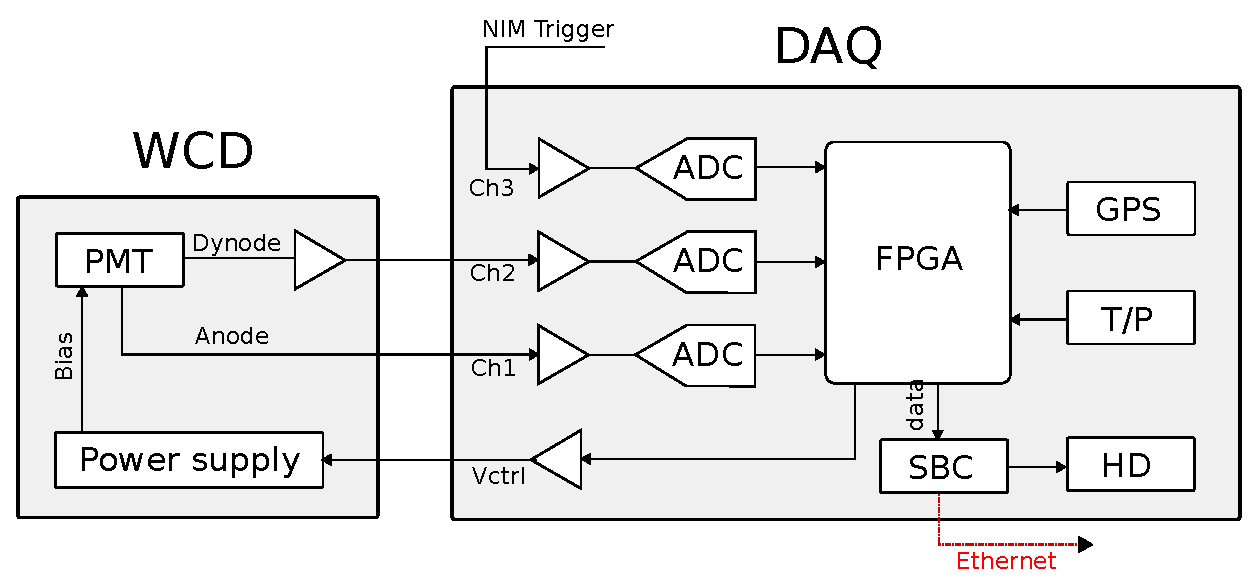
\includegraphics[width=0.9\columnwidth]{Figures/WCDDAQ.eps}
\caption{The diagram of the WCD DAQ system. The PMT and the bias electronics are inside the WCD. A 10 bits ADC digitizes signals from the PMT anode and last-dynode and stored in a hard disk join with temperature and barometric pressure data. An FPGA sets the acquisition parameters and the event time-stamp}
  \label{fig:WCD}
\end{figure}

In the WCD, a PMT R5912 detects the Cherenkov light from the charged particles crossing the water volume. The PMT is biased through a tapered resistive chain by a high-voltage power supply EMCO C20 spanning from $0$ to $2000$V. The pulses from the anode and the last dynode --amplified $20$ times-- are independently digitized by two $10$ bits ADCs with a sampling frequency of $40$ MHz. A $12-$sample vector stores the pulse shape in each channel,  when the signal amplitude exceeds the discrimination threshold ($\sim 100$ ADCU).  Then, a temporal label with $25$ ns resolution concatenates the event information. The timestamp is synchronized with the PPS signal from a GPS Motorola OnCore. Temperature and barometric pressure data are also recorded for the off-line analysis and data correction. An FPGA Nexys II handles the tasks of thresholding, base-line correction, temporal labelling, and temperature-pressure recording.

A third ADC channel digitizes a NIM signal coming from the hodoscope when an in-coincidence event occurs (See \ref{trigger}). The acquisition parameters of the WCD DAQ system (shown in Fig. \ref{fig:WCD} with discrimination thresholds and the PMT bias voltage) are set by an SCB Cubieboard 2. All the data is stored locally in an external hard disk. 

A central server collects (every 4 hours) data from the WCD and the hodoscope temporally in order to report the MuTe status towards a remote server via GSM. The local server, hodoscope, and WCD electronics are linked by an ethernet routing system as is shown in Fig. \ref{fig:power}. For working locally on the MuTe from an operator PC, a WiFi network is also established.


\subsection{Triggering system}
\label{trigger}
The MuTe triggering system determines events in-coincidence between the hodoscope and the WCD \cite{PeaRodrguez2019}. The Trigger T1 is individually enabled for the rear and frontal hodoscope panels when the pulse amplitude exceeds the discrimination threshold value. This trigger signal splits into three sublevels: the Trigger P1-P2 for cross-checking events in-coincidence and ToF measurements, the Trigger P1 for starting the data transmission from the MAROC 3A to the SCB, and the Ext-Trigger for holding the information inside the MAROC 3A while it is read.

For resolving the position of the activated pixel, MuTe accounts only the events activating a vertical and a horizontal bar per panel, called trigger T2. Events in-coincidence between the frontal and the rear panel in a time window of $7$ns to $12$ns classify as crossing particles, determine the trigger T3, and estimate the particle flux crossing the hodoscope. The coincidence window considers the time needed by a particle travelling at the speed of light through two critical paths: the shortest ($2.5$m) and the longest ($3.5$ m).

When the WCD detects a particle, the trigger T4 is activated. Next, the trigger T5 determines the events in-coincidence between the hodoscope and the WCD; this trigger is also called hybrid trigger (T5 = T3 \textbf{AND} T4). The NIM Trigger signal is digitized by the third ADC channel of the WCD for labelling the events in-coincidence with the hodoscope. All the time delays due to the transmission of the signals are considered for data analysis.

\subsection{Power consumption and operating autonomy}

\begin{figure}[htb]
\centering
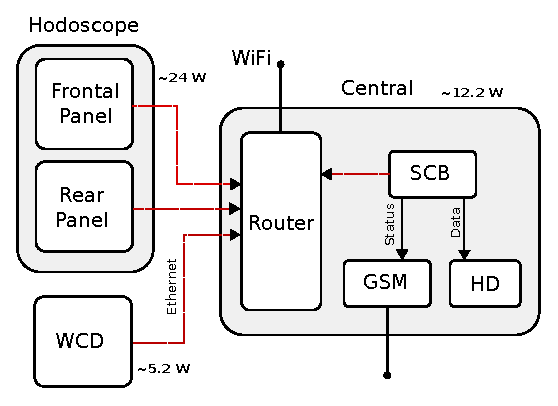
\includegraphics[width=0.6\columnwidth]{Figures/Total.eps}
\caption{General diagram of MuTe. The central server manages the data coming from the hodoscope and the WCD by a router while a central hard disk stores all the obtained data. For remote monitoring, MuTe sends its operational status via GSM. A WiFi connection link enables the possibility for local testing. The whole detector consumes $41.4$W where the central server dissipates the maximum power due to the hard disk, the intranet router, and the GSM transceiver.}
\label{fig:power}
\end{figure}

Electric consumption is a crucial parameter for our MuTe detector because it needs to operate autonomously on a distant location, and the energy system must provide enough power to avoid the detector shutdown. Thus, we have designed a photovoltaic system to give autonomy taking into account the power consumption of all the detector components. 

Figure \ref{fig:power} displays the power consumption schema of MuTe: $\sim 24$ W for the hodoscope,  $\sim 5.2$ W for the WCD  and $\sim 12.2$ W for the central monitoring server. The two hard disks  --used to store 470 MB per hour of data from the hodoscope and WCD-- are the devices with greater power consumption, but they provide almost six months of data-storage autonomy.

To estimate the power capacity and autonomy of the photovoltaic, we use meteorological information, i.e., irradiance, temperature, and cloudiness data from NASA satellites\footnote{National Aeronautics and Space Administration. Surface Meteorology and Solar Energy. \url{https://eosweb.larc.nasa.gov/cgi-bin/sse/sse.cgi?skip@larc.nasa.gov}} and from the Meteorology and Hydrology National Office\footnote{Instituto de Hidrología, Meteorología y Estudios Ambientales de Colombia. (IDEAM). Atlas Interactivo. \url{http://atlas.ideam.gov.co}} at typical volcano neighbourhoods in Colombia. The average irradiance per month for $22$ years is approximately $4-5$ kWh m$^{-2}$ day$^{-1}$ with an average temperature of $\sim 20^{\circ}$C and a maximum of $6$ consecutive cloudy days.

Several configurations of Victron Energy\footnote{BlueSolar polycrystalline panels (Datasheet). Taken from \url{https://www.victronenergy.com.es/upload/documents/Datasheet-BlueSolar-Polycrystalline-Panels-ES.pdf}.} photovoltaic panels were assessed. We found an optimum quantity of four panels of $100$W with a nominal voltage of $18$V, a nominal current of $5.56$A and a weight of $4.3$kg per panel.

The storage capacity required by the system in a day ($C_A$) is calculated using the modified Roger equation (\ref{cap_alma}) \cite{messenger2017photovoltaic}, i.e. 
\begin{equation}
C_a=\frac{E_c(1+F_s)}{\eta_{pb}\eta_{cdb}\eta_{rc}\eta_{pc}D_{b}} \label{cap_alma}
\end{equation}
where $E_c$ is the load energy considering DC/DC converters, $F_s$ the scaling factor, $\eta_{pb}$ the efficiency of conductors, $\eta_{cdb}$ the efficiency of batteries, $\eta_{rc}$ the battery charge and discharge efficiency, $\eta_{pc}$ the charge controller efficiency, and $D_{b}$ corresponds to the battery depth of discharge. $E_c$ defined as follows
\begin{equation}
E_c=E_x+\frac{E_{\gamma}}{\eta_{dcdc}}
\label{two}
\end{equation}
where $E_{x}$ is the load energy which does not require DC/DC converters, $E_{\gamma}$ the load energy requiring DC/DC converters and, $\eta_{dcdc}$ the efficiency of the DC/DC converters. From (\ref{two}) with $E_{x}=58.57$ Wh and $E_{\gamma}=746.24$ Wh, we have $E_c=844.08$ Wh. Therefore, by using $\eta_{pb}=0.97$, $\eta_{cdb}=0.95$, $\eta_{rc}=0.95$, $\eta_{pc}=0.98$, $D_{b}=0.8$ and $F_s=0.2$ (20\% oversizing), we can have a value of $C_a=1472.75$ Wh, while the total storage capacity with which the system will count can be obtained by means of
\begin{equation}
C_{at}=\frac{C_aD_a}{V_{nb}}
\end{equation}
where $D_a$ is the total number of autonomy days and $V_{nb}, $ is the nominal voltage of the battery bank. In this case, we set six days of autonomy with a nominal voltage of $12$V, resulting in a total storage capacity of $C_{at}=736.38$Ah. According to the criteria and environmental conditions presented above, we found the need for four batteries of $205$Ah with a weight of $65$kg per battery and a discharge depth of $80\%$.


\section{Mechanical response}
\label{mechanical}
\subsection{Structural design}
The hodoscope, the WCD, their electronics readout, and the central monitoring server are mounted on a sturdy metallic structure, as is shown in Fig. \ref{fig:Structure}. The frame consists of a $4.2$m $\times$ $2.8 m \times 1.8$m parallelepiped-shaped structure constructed of steel ASTM A-36 angles of $3.2$mm thick and mechanically attached by screws of 1/2 inch diameter. The MuTe inclination is set using a mobile base which can reach up to 15 degrees from the ground.

Figure \ref{fig:Structure} illustrates the structure of the instrument. Notice that the rear panel is fixed to one of the walls of the WCD, while the frontal panel can slide on a rail of $2.8$m length, providing a significant variable angular resolution for the telescope. 
\begin{figure}[htb]
\centering
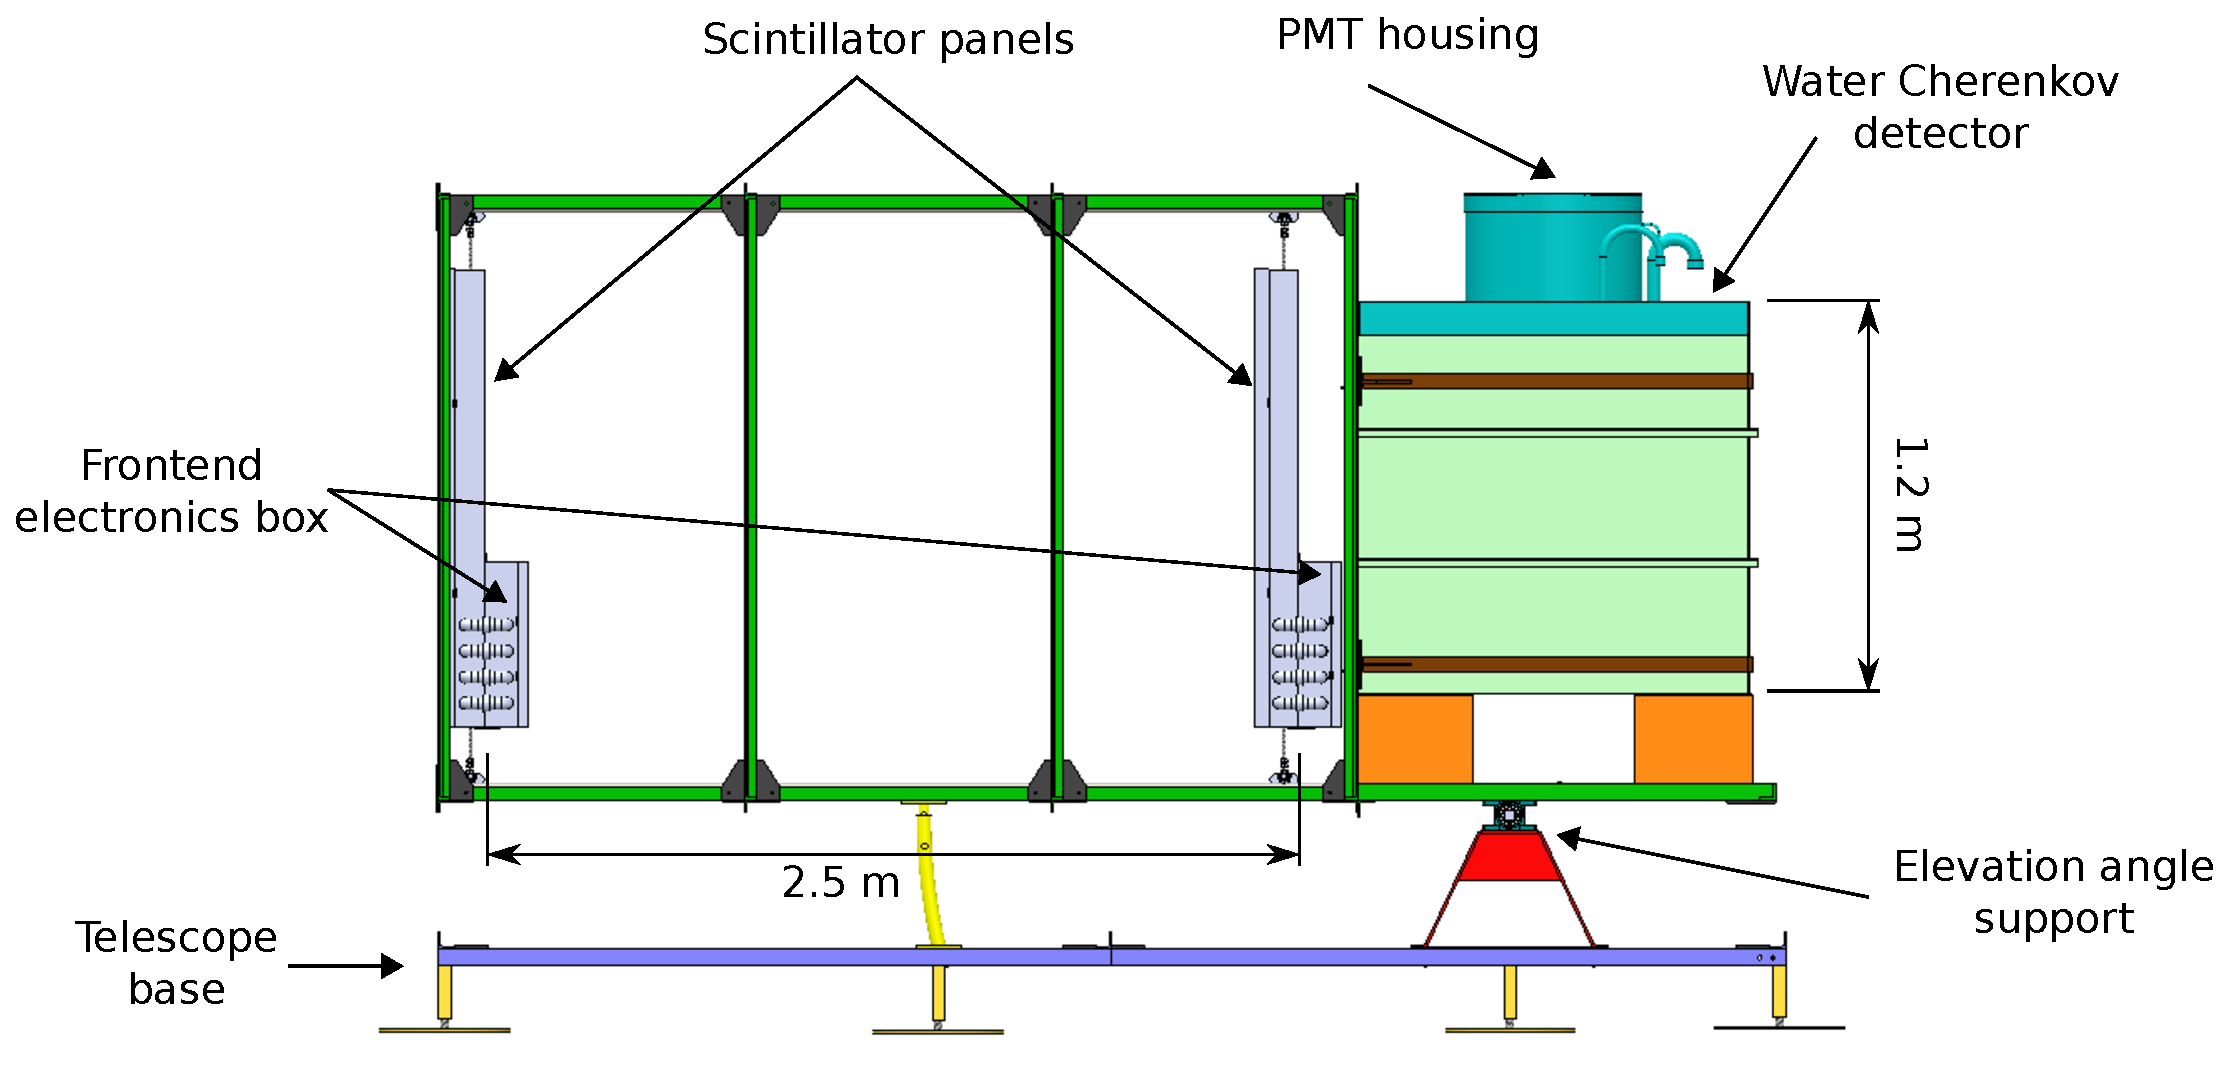
\includegraphics[width=1\columnwidth]{Figures/Detector.eps}
\caption{Lateral view of the MuTe detector. The WCD, placed on the center of mass of the structure, benefits the elevation movement which reaches up to $15^{\circ}$ by steps of $3^{\circ}$. The inter-panel distance can variate from  $40$ m up to $250$ m. The electronics front-end boxes are isolated from rain and humidity, as well as the PMT housing.}
  \label{fig:Structure}
\end{figure}

Since the MuTe will be working in field conditions inherent to volcanic environments,  it is necessary to study the mechanical behaviour of the detector under such conditions. For this reason, in the following section, we show the stress load and vibration analysis of the instrument, taking into account the structural design as well as mechanical stress due to tremors and wind conditions. Such simulations were performed using the \textsc{Solidworks 3D CAD Modeling Software} with the package \textsc{Solidworks Simulation} of structural analysis tools that use Finite Element Analysis (FEA) to predict real physical behaviour with linear, non-linear static and dynamic analysis capabilities.

\subsection{Vibrations analysis and tremors}
We calculate the natural frequencies and vibration patterns of the instrument from the dynamic response of the structure under external vibration wind sources. 

The area where the detector will be placed is compromised for the effects of the inherent dynamics of an active volcano. This means that ultimately, there could be tremors and movements of the internal structures of the volcano, which would cause earthquakes that would compromise the integrity of the instrument. Volcanic earthquakes are classified as: (a) volcano-tectonic earthquakes associated with fracturing that occur in response to stress changes in the active areas by fluid movement. Its frequency is generally with spectral peaks around 2-15 Hz. b) long period earthquakes with spectral peaks around 1-2 Hz attributed to resonance in cracks, cavities and ducts, due to pressure changes in fluids that exist in volcanoes \cite{mcnutt1992volcanic,londono2001spectral,langer2006automatic,chouet2003volcano}

\begin{table}[htb]
\begin{center}
\begin{tabular}{ccccc}
\hline
& {\bf Ang. frec.} & {\bf Frequency} & {\bf Min.}  & {\bf Max.}\\
{\bf Mode} & {\bf (Rad/s)} & {\bf (Hertz)} & {\bf (Hertz)} & {\bf (Hertz)} \\
\hline
1 & 10.053 & 1.6 & 0 & 0.01272\\ 
2 & 31.51 & 5.0149  & 0 & 0.0113 \\
3 & 35.465 & 5.6445  & 0 & 0.0303 \\
4 & 47.522 & 7.5633  & 0 & 0.0361 \\
5 & 47.565 & 7.5702 & 0 & 0.0166 \\
\hline
\end{tabular}
\end{center}
\caption{Natural frequency of vibration of the instrument.}
\label{Table_nat_frec1}
\end{table}

We exposed the instrument to five vibration modes, and the results obtained from the simulation are displayed in table \ref{Table_nat_frec1}. The structure reacts vibrating between a minimum and maximum frequencies, not exceeding $0.04$Hz, keeping the instrument safe against potential seismic events triggered by the volcano activity, which may range from $1.6$Hz to $7.5$Hz. The MuTe structure has a negligible mechanical affectation due to displacements caused by tremors or other movement manifestations inherent to volcanic environments.

\subsection{Static and wind load}
The analysis of static load aims to perform a simulation exploring the behaviour of the instrument structure against flexion, displacement, and deformation that can cause structural failures. 

The MuTe structure is composed mostly of steel ASTM A-36. The main possible effort for the structure emerges from two sources: the water volume inside the WCD ($\sim 1728$Kg) and the metal frames for the scintillator panels ($\sim 70$Kg each). The simulation mesh was $2.6 \times 10^6$ finite elements with $15 \pm 5$ mm size. Figure \ref{fig:stress} (left) displays the simulation results. The displacements range from  $0$mm up to $3.29$mm with the maximum peak stress under the WCD; however, such deformations do not represent any considerable mechanical problem for the instrument.
\begin{figure}[htb]
\centering
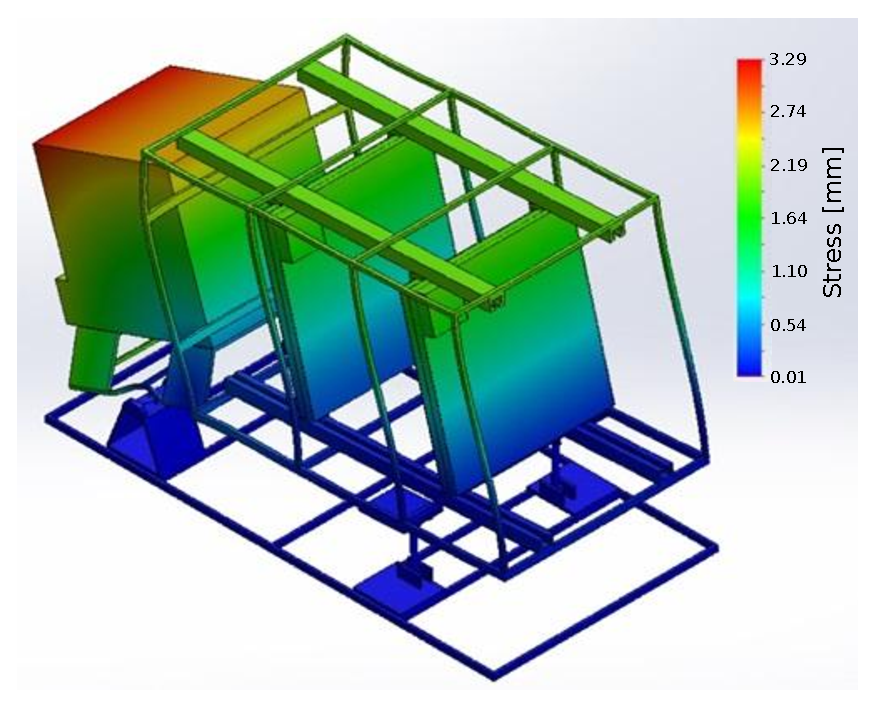
\includegraphics[width=0.48\columnwidth]{Figures/stress_graph.eps}
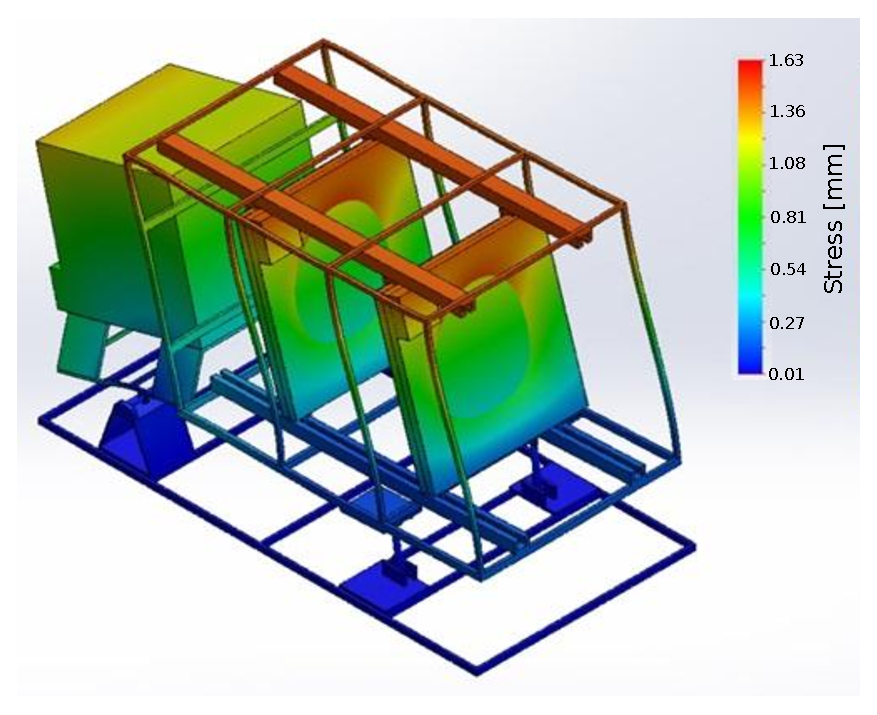
\includegraphics[width=0.48\columnwidth]{Figures/stress_graph_wind.eps}
\caption{Left and right plates illustrate the stress graph resulting from the static and dynamic --wind action-- load analysis, respectively. The maximum material deflection is about $3.29$mm in the rear part of the WCD, which is under high pressure due to the water weight.  The maximum pressure of wind occurs in the front of the scintillator panels suffering a mechanical displacement about $1.63$mm.}
\label{fig:stress}
\end{figure}


Additionally, to determine dynamical wind loads on the instrument, we use data from the Colombian Hydrology, Meteorology and Environmental Studies Institute \footnote{IDEAM by its acronym in Spanish of \textit{Instituto de Hidrología, Meteorología y Estudios Ambientales} \url{http://www.ideam.gov.co/}}. The maximum wind speed reported is $30$m/s, with an occurrence probability of $4\%$.

% \begin{figure}[htb]
% \centering
% 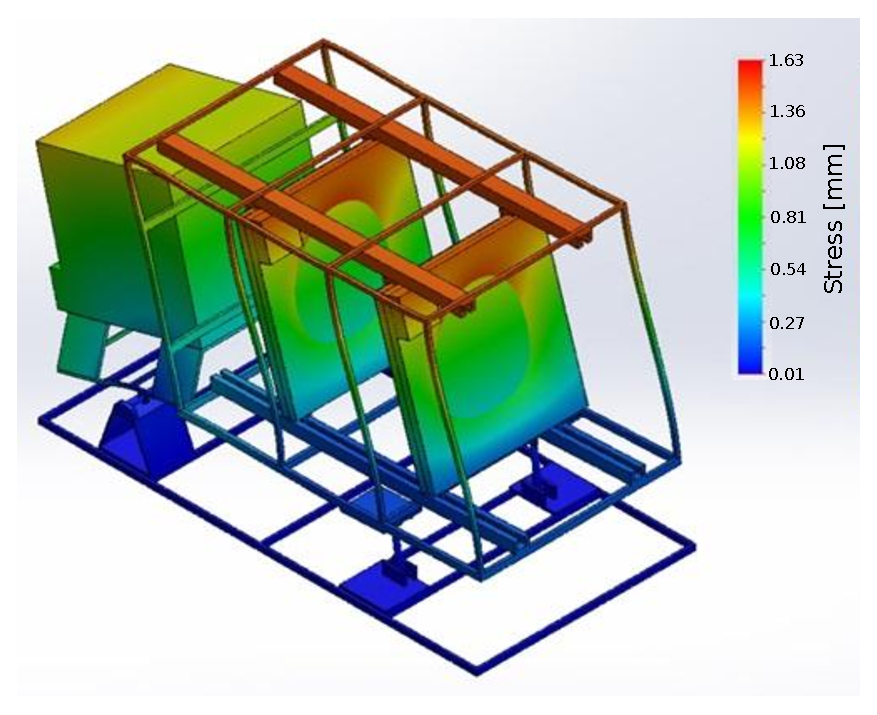
\includegraphics[width=0.6\columnwidth]{Figures/stress_graph_wind.eps}
% \caption{Stress graph resulting of the dynamic load analysis by wind action. The maximum pressure of wind occurs in the front of the scintillator panels suffering a mechanical displacement about $1.63$ mm.}
% \label{fig:stress_wind}
% \end{figure}

The right panel in figure \ref{fig:stress} illustrates the structure stress due to wind load. The mechanical structure suffers displacements up to $1.63$mm in the frontal part of the scintillator panel. However, this displacement is not representative, and the instrument will not experience significant deformations.

\subsection{Heat dissipation in the structure}
We compute the temperature distribution in the MuTe based on the thermal inputs (heat loads) and thermal outputs (heat losses) taking into account conduction, convection and thermal irradiation present in the detector environment. Such processes involve environmental temperature, solar radiation, cooling by wind, and heating by electronics power consumption.

The thermal analysis allows us to know the heat transfer along with the structure and how it may affect the detector components. Instrument safety and functioning on the field is an essential factor to take into account since many materials in the detector have properties that depend on temperature such the SiPMs and scintillator bars.

We performed the thermal analysis of the structure with the heat module of \textsc{Solidworks Modeling Software}. The parameters in Table \ref{instr_mat} were taken into account for computing the temperature distribution on the MuTe structure. The average temperature, radiation and wind speed on the observation place were provided by the IDEAM.

From Fig. \ref{fig:temp_graph}, we can see that the maximum temperature in which the detector is subjected is around $60^{\circ}$C located in the centre of the scintillation panels where a large surface is heated by the solar radiation, while there is an average of $23^{\circ}$C in the rest of the structure. The WCD, although it has a large metallic surface, represents a good source of heat dissipation because of its water content ($1.7$ m$^3$) finding a maximum temperature of $40^{\circ}$C. On the other hand, the frontal side of both panels has a lower temperature than the rear side since the wind flow generates a cooling process by convection. 

\begin{table}[!ht]
\begin{center}
\begin{tabular}{ll|ll}
\hline
\multicolumn{2}{c}{\bf DETECTOR MATERIALS} & \multicolumn{2}{|c}{\bf HEAD SOURCES DATA}\\
\hline
Structure Material: & AISI 1020 & Sky temperature & -10 $^{\circ}$C \\
Model type: & Linear elastic isotropic & Electronic box WCD & 5.2 W \\
Thermal conductivity: & 47 W/(m K) & Gen. electronic box & 12.5 W \\
Specific heat: & 420 J/(kg K) & Electronic box Scint. & 12.3 W \\
Density: & 7900 kg/m$^3$ & Sun radiation & 4500 Wh m$^{-2}$ day$^{-1}$ \\
Cherenkov medium: & Water & Convection coeficient & 10 W/(m$^2$ K) \\
Model type: & Linear elastic isotropic & Mean enviroment temp. & 16 $^{\circ}$C \\
Thermal conductivity: & 0.61 W/(m K) & Base water temperature & 10 $^{\circ}$C \\
Specific heat: & 4200 J/(kg K) & & \\
Density: & 1000 kg/m$^3$ & & \\ 
\hline
\end{tabular}
\end{center}
\caption{Instrument materials and basic data used in a model of heat analysis.}
\label{instr_mat}
\end{table}

\begin{figure}[htb]
\centering
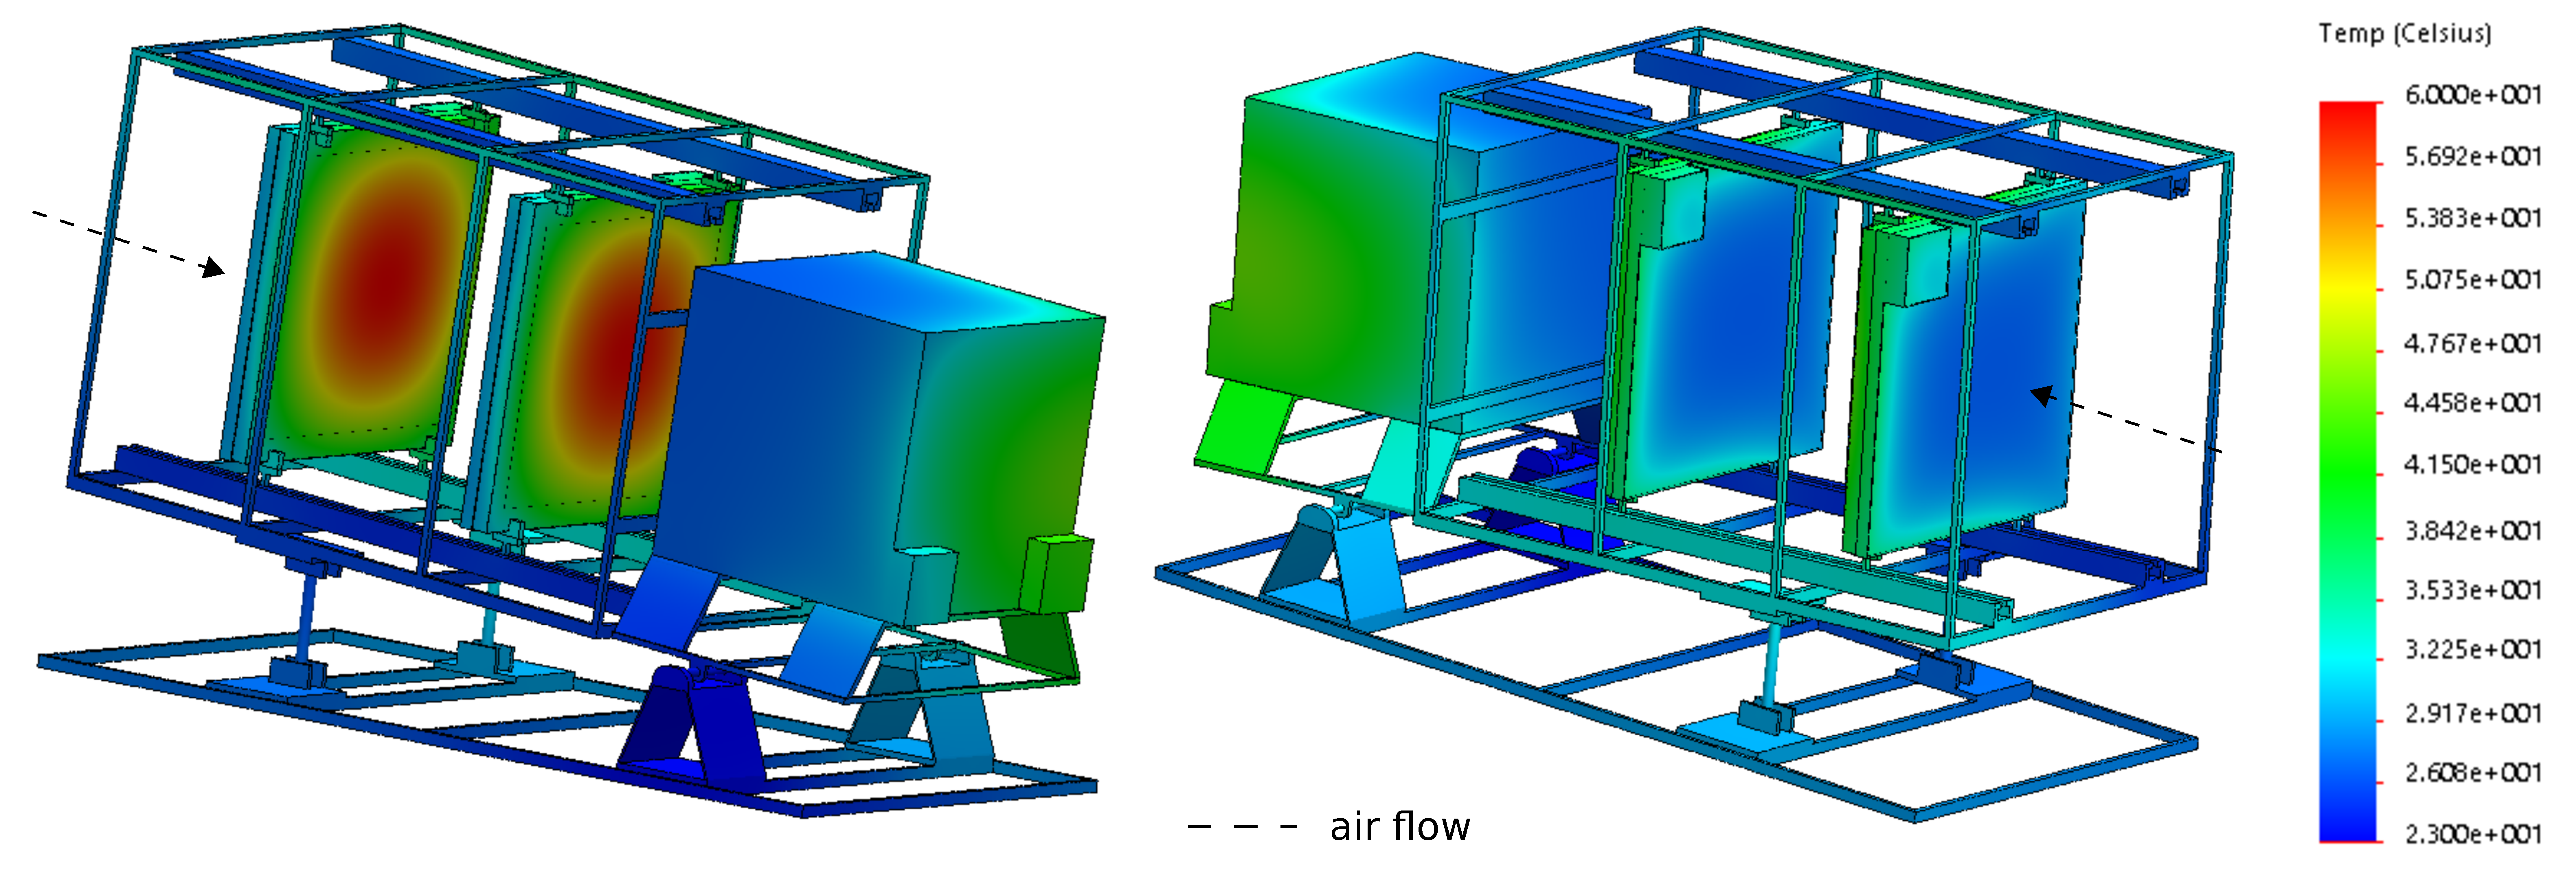
\includegraphics[width=1\columnwidth]{Figures/MuTe_Temp.eps}
\caption{Temperature distribution of MuTe. The maximum heating point ($60^{\circ}$C) is on the rear side of the scintillator panels due to the solar radiation, while the frontal side of them is cooled by wind convection. The WCD has its heat-dissipation mechanism due to its water volume content.}
\label{fig:temp_graph}
\end{figure}

The temperature distribution allows distinguishing the critical heating points in the detector structure. Consequently, we can adjust the heat dissipation using accessories such as a tent to isolate the instrument from solar radiation but with the possibility of air circulation to conserve heat transfer by convection. 

\section{First measurements}
\label{measurement}
The MuTe hodoscope recorded its first measurements during $15$hours, with the average count rate by scintillator bar roughly $836.3$ event/h and a discrimination threshold of $8$photo-electrons. The inter-panel distance was $134$cm, the angular aperture of $82^{\circ}$ and a maximum acceptance value of $12.83$cm$^{2}$sr.  To reconstruct the particle trajectories and the flux crossing the hodoscope, we apply a four-bar activation condition: a pair XY in the frontal panel and a pair XY in the rear one. However, we must correct the measured flux by a scale factor of $112.9$resulting in the minimum condition of coincidence (activation of one bar in the frontal panel and one in the rear one). 

\begin{figure}[htb]
\centering
\includegraphics[width=0.48\columnwidth]{Figures/Hits_15h.png}
\includegraphics[width=0.49\columnwidth]{Figures/Flux.png}
\caption{Particle count measured by the hodoscope during 15 hours for a separation between planes of $D=134$ cm. For this experiment a flux of 10.7 $\times 10^{-3}$ cm$^{-2}$sr$^{-1}$s$^{-1}$ corresponding with vertical directions is measured. As it is expected, the flux decreases while the zenith angle increases. For a zenith angle of 41 $^{\circ}$ the flux is around 4.5 $\times 10^{-3}$ cm$^{-2}$sr$^{-1}$s$^{-1}$, half order of magnitude lower than the flux maximum.}
\label{fig:hits_15}
\end{figure}

In Fig. \ref{fig:hits_15} we show the number of hits and the particle flux recorded by the hodoscope. The maximum number of hits was around 67 for perpendicular trajectories ($\theta_x=\theta_y=0^{\circ}$) respect to the hodoscope plane. The number of events decreases for inclined trajectories due to the hodoscope acceptance shape and the muon flux which is modulated by the zenith angle ($\cos^2 \theta$). The estimated flux reaches up a maximum of 10.7 $\times 10^{-3}$ cm$^{-2}$sr$^{-1}$s$^{-1}$ which is comparable with the flux obtained by \textit{Lesperre} \cite{Lesparre2012} of 9 $\times 10^{-3}$ cm$^{-2}$sr$^{-1}$s$^{-1}$. The variance in the flux histogram can be reduced by increasing the acquisition time.

The MuTe was set to 90$^{\circ}$ zenith (0$^{\circ}$ of elevation) as it is shown in Fig. \ref{fig:WCDHod} in outdoor conditions. The WCD and the hodoscope act as individual detectors but synchronized in time. The flux in-coincidence between the hodoscope and the WCD is two orders of magnitude lower than all the events recorded by the WCD, representing only 2$\%$ as is shown in the deposited energy histogram in Fig. \ref{fig:WCDHod_rate}. This flux reduction mainly occurs due two factors: the muon flux is almost 2 orders of magnitude weaker at quasi-horizontal angles than the maximum flux at 0${\circ}$ zenith, furthermore, the angular acceptance of the WCD is roughly 2$\pi$ while the acceptance of the hodoscope is only a fraction of that, constrained by the coincidence between both sensitive panels.

\begin{figure}[htb]
\centering
\includegraphics[width=0.7\columnwidth]{Figures/Acceptance.eps}
\caption{MuTe setup first on-field measurements. The detector is pointing towards the horizon with an elevation angle of $0^{\circ}$. The aperture of the hodoscope $\theta_H$ is $50^{\circ}$ for a separation distance between panels of $250$cm. The aperture of the whole detector (WCD + hodoscope) $\theta_C$ is roughly $32^{\circ}$.}
\label{fig:WCDHod}
\end{figure}

%voy por aquí
The deposited energy histogram of the WCD-hodoscope data is composed by three sources: muons, electron/positrons and multiple particle events. The muonic component represents roughly the 33.6$\%$ of the events ($180$ MeV $< E_{loss} < 400$ MeV), the electromagnetic $36$\% ($E_{loss} < 180$ MeV), and the multiple particle $30.4\%$ ($E_{loss} > 400$ MeV) of the histogram. 

\begin{figure}[htb]
\centering
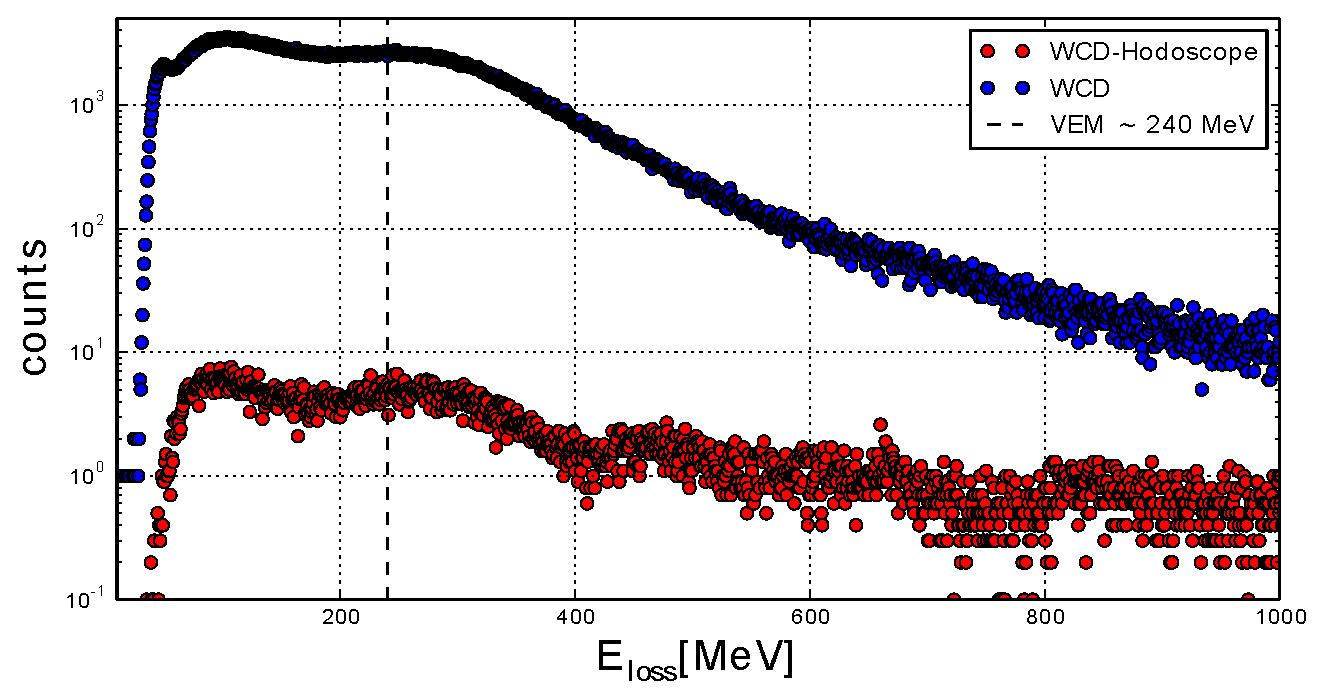
\includegraphics[width=0.7\columnwidth]{Figures/WCDHod.eps}
\caption{WCD deposited energy histogram for the omnidirectional events detected by the WCD (blue) and for the events in-coincidence between the WCD and the hodoscope (red). The dashed line represents the deposited energy of the vertical muons (VEM) which is estimated to be $240$MeV taking into account muon losses about $2$MeV/cm in water. The first hump corresponds to the energy deposited by electrons, positrons and gammas while above $400$MeV events correspond to multiple particles.}
\label{fig:WCDHod_rate}
\end{figure}

These results show how the noise background (electromagnetic and multiple particles) is comparable to the signal, even greater taking into account that soft muons have not been extracted from the muonic component. On the other side, multiple particle background, which is made by several particles temporally correlated, e.g. inclined cosmic showers impacting the detector \cite{Bonechi2019}, become more significant comparing it with the magnitude of the electromagnetic and muonic humps.

\begin{figure}[htb]
\centering
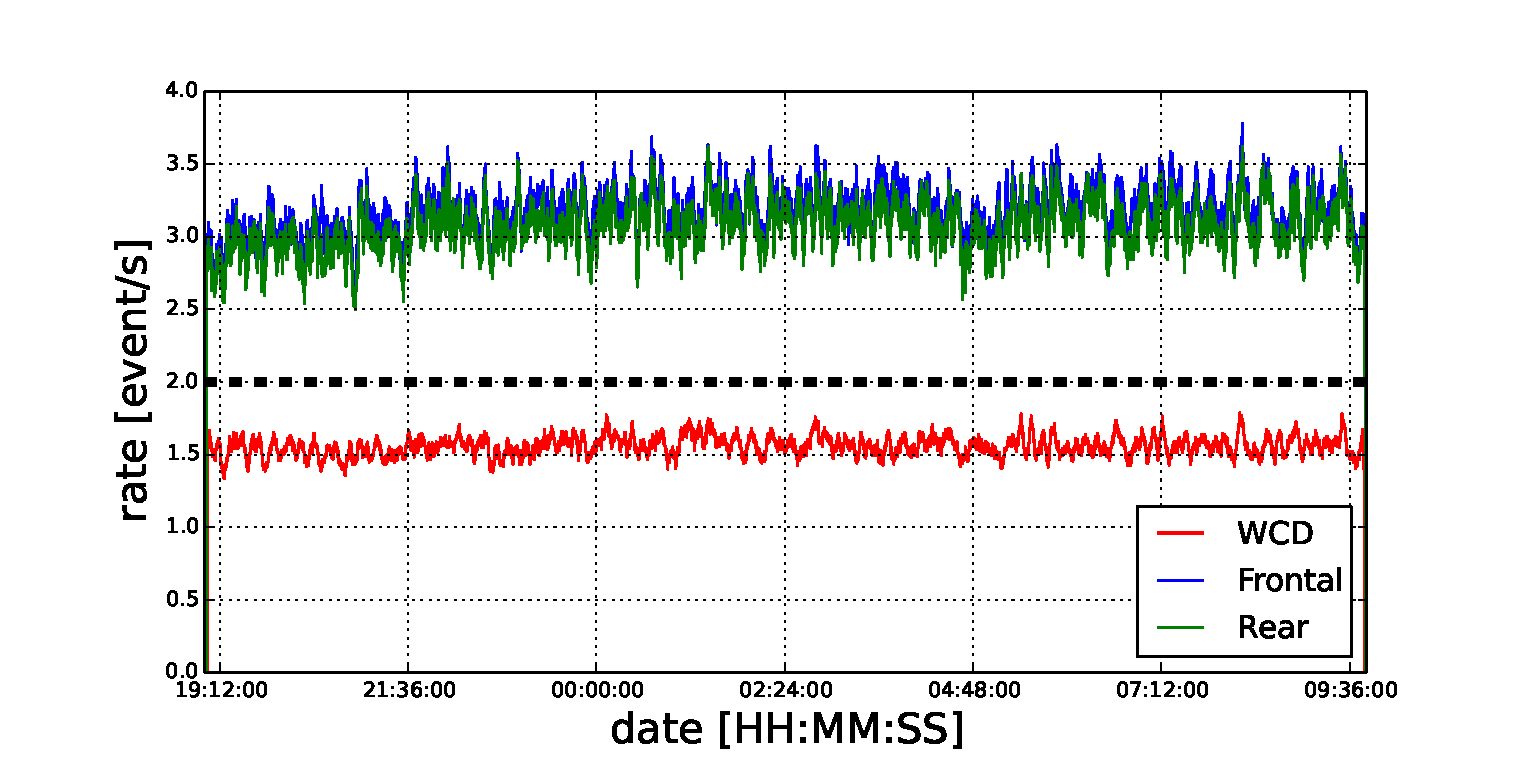
\includegraphics[width=0.8\columnwidth]{Figures/HodWCDRate.eps}
\caption{Event rate detected by the front (blue), rear (green) and the WCD (red) in-coincidence. The WCD rate is $50\%$ lower than the detected by the panels due to it is not able to measure particles coming from trajectories at high inclination angles respect to the hodoscope plane. The dashed line indicates the expected WCD rate taking into account the ratio between the angular apertures $\theta_H$ and $\theta_C$.}
\label{fig:RateWCDH}
\end{figure}

The aperture angle of the hodoscope $\theta_H$ at an inter-panel distance of $2.5$m is around $50^{\circ}$, and the aperture of the whole detector (WCD + hodoscope) $\theta_C$ is roughly $32^{\circ}$. That means, some trajectories having very inclined angles can not be detected by the WCD. The WCD identifies the $62\%$ of the hodoscope events. In Fig. \ref{fig:RateWCDH} we show the coincidence rate detected by the hodoscope planes and the WCD during $14$hours. The mean rate for the panels is around 3.2 events/s and for the WCD 1.5 events/s, which represents the $50\%$ of the hodoscope and it is lower than expected due to the detection efficiency.


\section{Discussion and conclusions}
\label{conclusions}
%Muons are charged particles that can penetrate several kilometers of Earth's crust and their absorption rate depends on the material density they are crossing. Nowadays, muography can solve inner characteristics of structures with a resolution up to tens of meters. However, its practical use requires a good knowledge of the dependencies between spatial and angular resolution, acquisition time, target size and distance between the target and the detector. To extend the performance capabilities of muography it is necessary to address all these aspects at a design level taking into account results from simulations and experimental verification.

In this paper we have presented the design and simulation of a muon telescope prepared for making density measurements in volcanoes located in the central mountain range of Colombia using muography. Our design includes an hodoscope formed by a pair of detection matrices made of plastic scintillators for the determination of the trajectories of muons crossing the volcanic structure. The hodoscope reaches up an angular resolution of 32 mrad for a inter-panel distance of 250 cm. Furthermore, our design also incorporates particle identification techniques in order to filter background sources in muography. A water Cherenkov detector allows to reduce noise signals coming from the soft-component of EAS (electrons and positrons), and multiple particle events by means of energy loss estimation. The WCD also measures fluctuations in the cosmic ray background at the observation place. Additionally, a picosecond Time-of-Flight system measures the direction and momentum of incident charged particles allowing to remove back-coming and low momentum scattered muons. We estimated MuTe is able to discriminate muons under 0.6$\pm$0.1GeV/c taking into account the 40 ps ToF resolution.

The background noise due to the electromagnetic component of EAS was estimated to be 36$\%$. The events caused by muons represent about 33.6$\%$ of the collected data, containing backward muons, low momentum muons, and crossing muons. The multiple particle noise was 30.4$\%$ being two-particle events the most probable in comparison with events involving more simultaneous particles. Such events release an average energy of 480 MeV in the WCD. 

The integral flux recorded by the hodoscope pointing at 90$^{\circ}$ with an aperture of 82$^{\circ}$ drops drastically about to orders of magnitude in relation to the total integral flux recorded by the WCD at the observation place. Such flux drop allows the multiple particle noise to become more significant, decreasing the detector SNR.

After performing a complete analysis of the MuTe mechanical response against vibrations and tremors ranging from 1.6 to 7.5 Hz, we found the MuTe structure has no serious affectation. On the other hand, the maximum temperature in the hodoscope under environmental conditions was 60$^{\circ}$ in the rear side of the scintillation panels. An average wind speed of 30 m/s generates a convection process in the front side of the panels causing a temperature drop until 23$^{\circ}$. The WCD temperature is regulated by its water content reaching up to 40$^{\circ}$. The thermal analysis was taken into account for optimizing the SiPM functioning. Such results are exposed in a manuscript under preparation.


%A big challenge for the MuTe is to carry out {\it in situ} measurements of the atmospheric muon flux attenuation after crossing volcanic edifices at locations with complicated topography characteristics and adverse tropical environmental conditions (humidity, temperature variations, and wind currents). To ensure a good performance of the instrument we have considered a series of mechanical simulations taken into account the detector structural features for operating in long periods of time. 

%Therefore, determining and modelling volcano inner structures is crucial to evaluate their potential risk. This might be achieved through a powerful technique such as muography, which measures the muon flux attenuation by rock volumes of different densities allowing the imaging of volcanic conduits inside the volcanic edifice. It constitutes an engaging way to infer density distributions inside geological structures, which is critical for studying magma dynamics associated to possible eruptive scenarios. 


\acknowledgments
This research was carried out as part of the Muon Telescope project on {\it Grupo de Investigaci\'on en Relatividad y Gravitaci\'on} (GIRG) under financial support of  Departamento Administrativo de Ciencia, Tecnolog\'ia e Innovaci\'on of Colombia (ColCiencias) under contracts FP44842-051-2015 and FP44842-661-2015. DSP would like to thank GIRG, Grupo Halley and Vicerrector\'{\i}a Investigaci\'on y Extensi\'on Universidad Industrial de Santander for the hospitality during my post-doctoral fellowship.

The research group is grateful to have the experience and advice of the Servicio Geologico Colombiano - SGC who have participated and worked together in the phase of determining the best sampling sites taking into account the design and transportability conditions of our detector.


\bibliographystyle{unsrt}
\bibliography{MuTe_bib.bib}

\end{document}

In summary, the simulations of load distribution by weight and wind have shown that the mechanical design of MuTe is robust. The maximum stress values for static and dynamical loads do not represent a risk for the detector structure and electronics system maintaining it safe while functioning.